\clearpage

\subsection{Liposomal structures} ~\\
\label{plugin:vesicle}

In this section some specialized spherical multi-shell structures are summarized which describe a few types of liposomal vesicular structures. The main characteristics of a vesicle are shown in fig.\ \ref{fig:liposomal_vesicular_structure}. In first approximation these vesicles are described as spherical shell structures, where the lipid hydrophobic tail groups from the core of the spherical membrane and the hydrophilic head groups the inner and outer shell of this spherical membrane. This containment has aqueous solution inside and outside. As the lipids are in general very well known one likes to extend the models of a bilayer as described in section \ref{sect:BilayeredVesicle} or \ref{subsubsect:EllSh+SD+BiLayerGauss} by known  molecular constrains like in section \ref{subsect:DiblockCopolymerMicelles} about diblock copolymer micelles.

\begin{figure}[htb]
\begin{center}
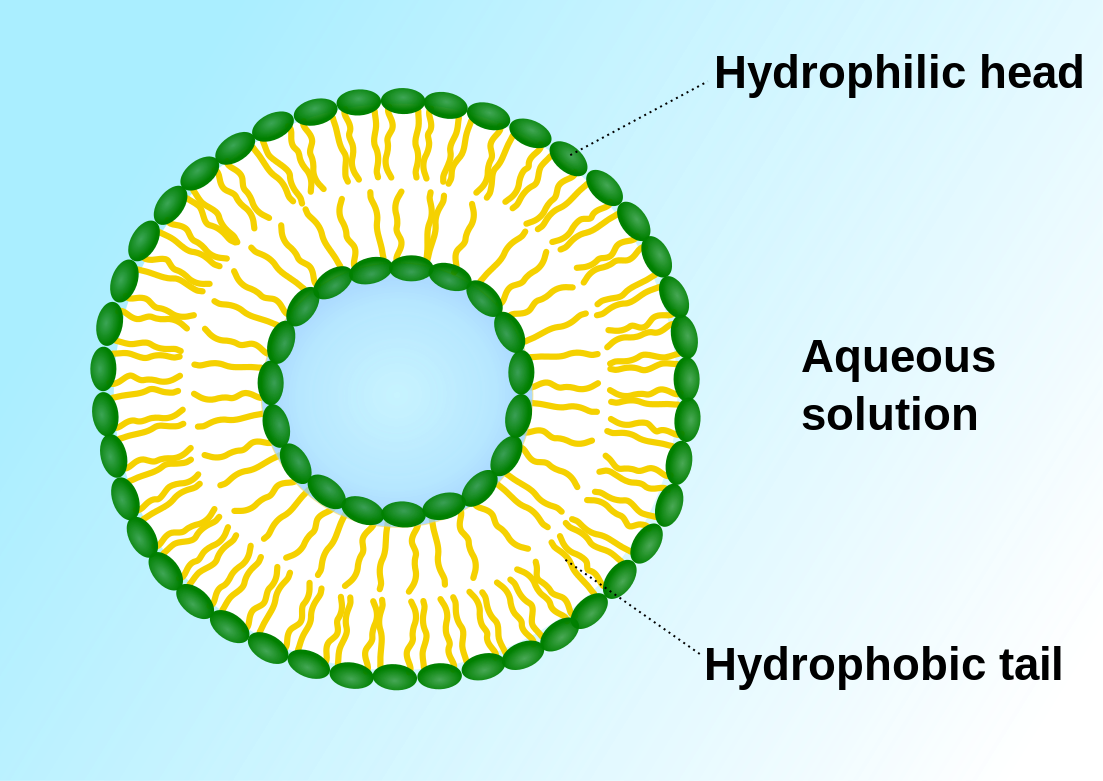
\includegraphics[width=0.8\textwidth]{../images/form_factor/vesicles/Liposome_scheme-en.png}
\end{center}
\caption{scheme of a liposomal vesicular structure}
\label{fig:liposomal_vesicular_structure}
\end{figure}

\begin{figure}[htb]
\begin{center}
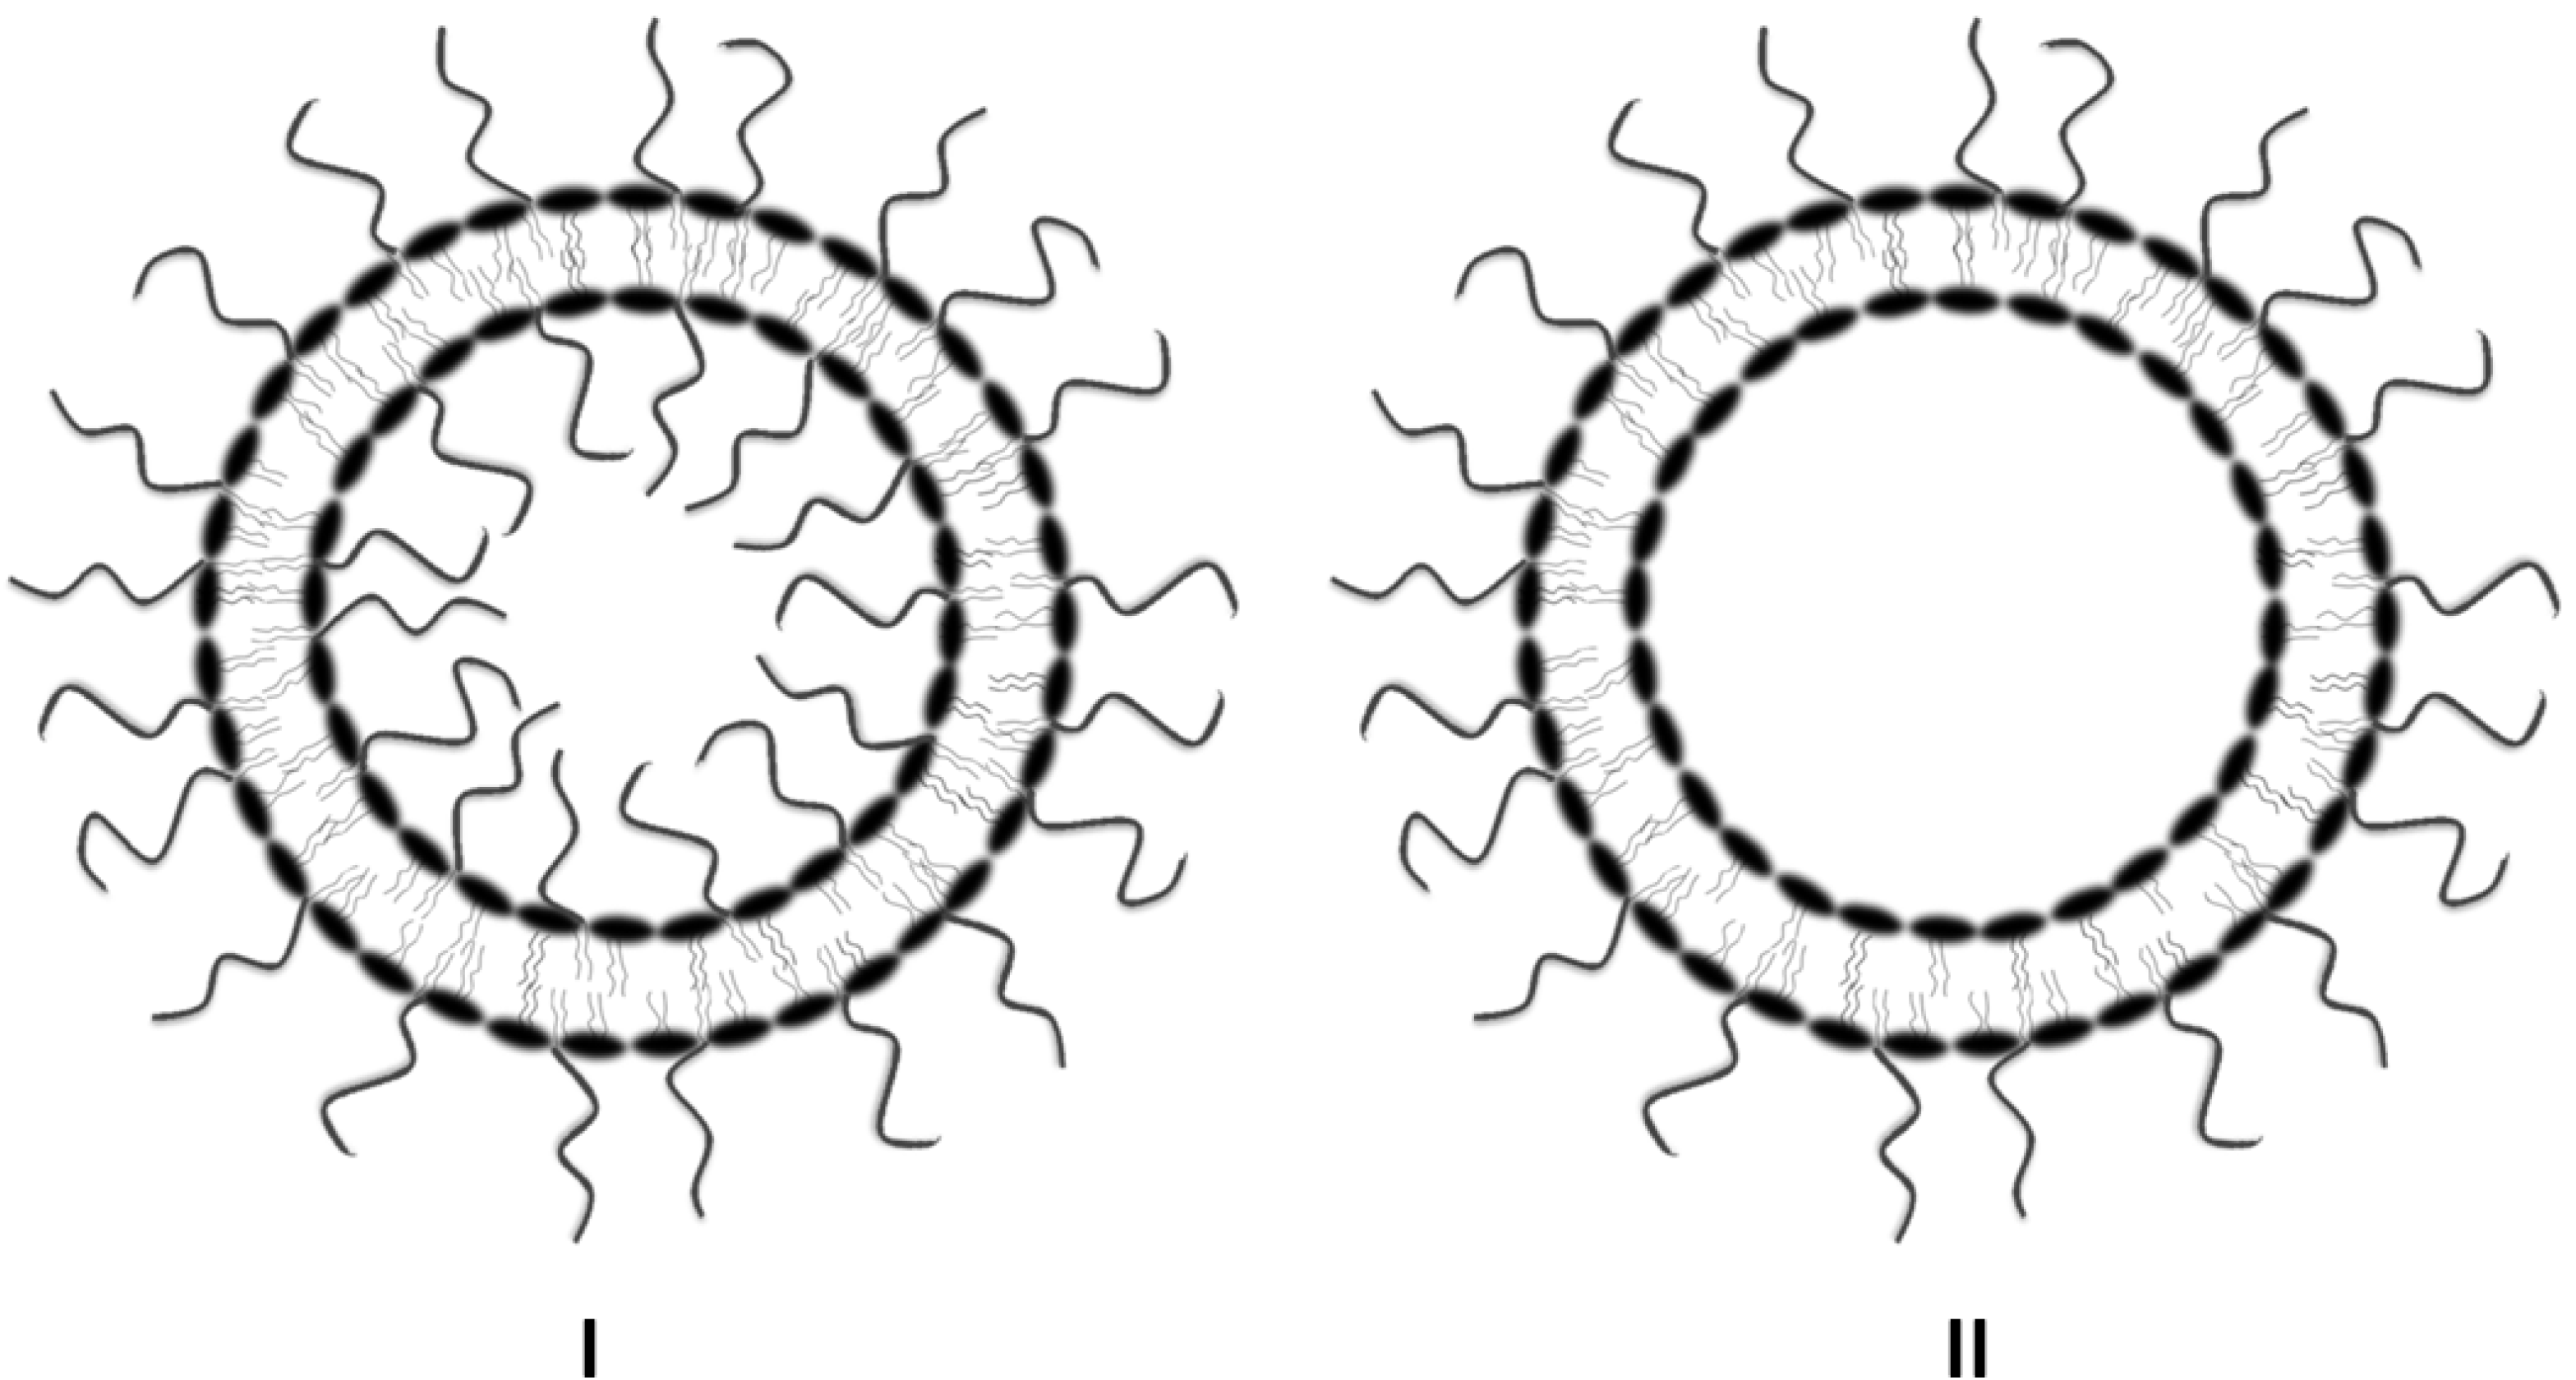
\includegraphics[width=0.8\textwidth]{../images/form_factor/vesicles/pegylated_liposome.png}
\end{center}
\caption{scheme of pegylated vesicle with PEG molecules both inside and outside or only outside the vesicle}
\label{fig:pegylated_vesicle}
\end{figure}

In pharmaceutical applications these vesicles are decorated with PEG molecules to increase their circulation time in a living body, as they give them a sort of stealth properties against the immune system. depending on the synthesis procedure the PEG molecules are either attached on both sides or mainly from the outside as shown in fig.\ \ref{fig:pegylated_vesicle}.

The dimension in the vesicle are typically such, that the thickness of the bilayer is much smaller than the overall diameter of a micelle. Therefore next to a full 3D Fourier transform of the scattering length density profile also an approximation factorizing the contribution of the small object dimension and from the large object dimension can be performed. For very thin random orientated particles the form factor can be factorize according to Porod \cite{Porod1948} in a cross
section term $P_\text{cs}(Q)$ for the shorter or thin dimension and a shape factor $P'(Q)$ for the long dimension. For a small number of of cross-section types and shapes such functions are suppled in section \ref{plugin:Pcs4planar} and \ref{plugin:Pprime4planar} developed to describe the scattering of local planar objects.

~\\

\subsubsection{PEGylated liposome with piecewise constant bilayer scattering length density profile} ~\\

This version of a pegylated vesicle is following the formalism used in \cite{Arleth2010} and \cite{Nielsen2018}.

~\\
\subsubsection{PEGylated liposome with approximate gaussian scattering length density profile} ~\\

In practise it could be shown \cite{Pabst2002,Brzustowicz2005} that at least for x-rays the scattering length density profiles across a membrane are better modelled by a gaussian scattering length density profile. 